\section{\secsumprod}
\label{sec_model_sum_prod}

We start this section with two activities that involve modeling with sums.  Next, we look at modeling with sums and products and introduce a notation for writing general sums and products without using ellipses ($\ldots$).  

%%%%%%%%%%%%%%%%%%%%%%%%

%Appears in \Cref{sec_sums_and_products}.

\newcommand{\subhowmanysq}{Counting Squares}
\subsection{\subhowmanysq}
\label{sub_how_many_squares}

We begin with an activity that involves a sum.

\begin{act} [Counting Squares]
\label{act_how_many_sq_puzzle}
~
    \begin{actpart}
        \item How many squares appear on the standard chessboard as drawn in \Cref{fig_chessboard_hms}?  
        
        Hint:  There are 64 $1 \times 1$ squares, one $8 \times 8$ squares, and many more squares of other sizes.  Show the steps of your calculation in an organized manner and clearly indicate your final answer.

        \begin{figure}[hbtp]
            \centering
            \scalebox{.5}{% \begin{tikzpicture}[x=1cm]
% \foreach \y in {0,2,4,6}{
%     \foreach \x in {0,2,4,6}{
%         \fill (\x,\y) rectangle (1+\x,1+\y) rectangle (2+\x,2+\y);}}
% \end{tikzpicture}

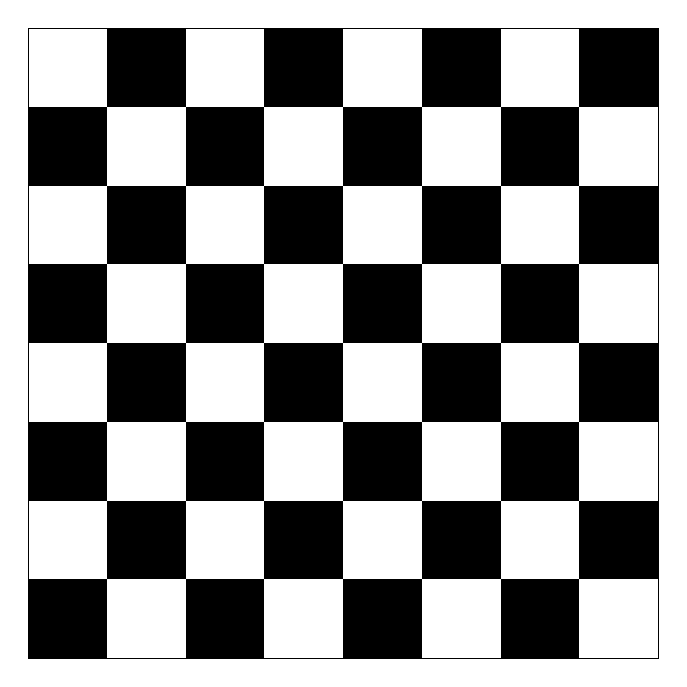
\begin{tikzpicture}[x=1cm]
    \foreach \x in {0,...,7} \foreach \y in {0,...,7}
    {
        \pgfmathparse{mod(\x+\y,2) ? "white" : "black"}
        \edef\colour{\pgfmathresult}
        \path[fill=\colour] (\x,\y) rectangle ++ (1,1);
    }
    \draw (0,0)--(0,8)--(8,8)--(8,0)--cycle;
\end{tikzpicture}}
            \caption{The standard chessboard.}
            \label{fig_chessboard_hms}
        \end{figure}

        \item Conjecture the number of squares on an $n \times n $ chessboard.  
    \end{actpart}
\end{act}

Let's take a closer look at \Cref{act_how_many_sq_puzzle}.

\begin{exam}[Counting $ \times 5$ squares]
\label{exam_count_5x5sq}
    How many $5 \times 5$ squares are there on the $8 \times 8$ chessboard?
        \begin{soln}
            Think of taking a $5 \times 5$ square and moving it around on top of the $8 \times 8$ square.  If we start with a the $5 \times 5$ square in the upper left hand corner, we can move it one, two, or three units to the right. That is, there are four $5 \times 5$ squares that fit along the top row.  If we move it down one unit, there are also four $5 \times 5$ squares that fit one row down. Similarly, there are four $5 \times 5$ squares that fit two rows down and four $5 \times 5$ squares that fit three rows down. That is the furthest we can go, so there are $4+4+4+4=16$ different $5 \times 5$ squares.

            There is a more sophisticated way to count.  We can create a pairing between each possible $5 \times 5$ squares and its upper left-hand corner, which is a $1 \times 1$ square.  Which $1 \times 1$ squares can be the upper left-hand corner of a $5 \times 5$ square?  The answer is any $1 \times 1$ squares in the $4 \times 4$ square that sits in the upper left-hand corner of the $8 \times 8$ chessboard.  (If we try to put the upper left-hand corner of the $5 \times 5$ square anywhere else on the chessboard, then the $5 \times 5$ square will not fit.)  Because we have a pairing, the number of $5 \times 5$ squares equals the number of $1 \times 1$ squares in the $4 \times 4$ square that sits in the upper left-hand corner of the $8 \times 8$ chessboard.  Since any $4 \times 4$ square has exactly $4^2=16$ of the $1 \times 1$ squares, the answer again is $4^2=16$.
        \end{soln}
    
\end{exam}

%%%%%%%%%%%%%%%%%%%%%%%%%%%%

\newcommand{\subfactrep}{Factorial Representations}
\subsection{\subfactrep}
\label{sub_factorial_rep}

In this puzzle, we represent an integer by writing it as the sum of factorials.  
\begin{act}[Factorial Representations Puzzle]
\label{act_fact_rep}
    As a reminder, the first few factorial are listed in \Cref{tab_factorials_1to8}.

        \begin{table}[hbtp]
            \centering
            \begin{tabular}{cccc}
                $1! = 1$ & $2! = 2$ & $3! = 6$ & $4! = 24$ \\
                $5! = 120$ & $6! = 720$ & $7! =$ 5,040 & $8! = $40,320
            \end{tabular}
            \caption{The values of $n!$ for $n=1,2, \ldots 8$.}
            \label{tab_factorials_1to8}
        \end{table}
    Every positive integer can be written as the sum of factorials. For example, we can write 10 using $3!=6$, $2!=2$, and $1!=1$ in several ways, including
        \begin{align*}
            10 &= 1 + 1 + 1 + 1 + 1 + 1 + 1 + 1 + 1 + 1  \\
            &= 2 + 2 + 1 + 1 + 1 + 1  \\
            &= 6 + 2 + 1 + 1 \\
            &= 6 + 2 + 2    
        \end{align*}
    The last line uses the fewest factorials.  When we write the positive integer $n$ using the fewest factorials, that is the \textbf{factorial representation} of $n$. 

    There is a handy shorthand for this notation.  For example, the factorial representation of 10 is
        $$10 = 6 + 2 + 2 = \underline{1} \cdot 3! + \underline{2} \cdot 2! + \underline{0} \cdot 1! =(120)_!$$
    For example, 
        $$(10320)_! 
        = \underline{1} \cdot 5!
        + \underline{0} \cdot 4!
        + \underline{3} \cdot 3!
        + \underline{2} \cdot 2!
        + \underline{0} \cdot 1!
        = 120 + 3(6) + 2(2) = 142.$$

    \begin{actpart} 
        \item Evaluate $(1201)_!$ % 24+12+1=37
        \item Evaluate $(1000)_!$ and $(10000)_!$.  What do you notice?
        \item Find the factorial representation of 5, 20, and 132.
        
        \item  A classmate is writing the factorial representation of 27 and her answer is 
            $$ 27 
            = 6 + 6 + 6 + 6 + 2 + 1 
            = \underline{4} \cdot 3! + \underline{1} \cdot 2! + \underline{1}\cdot 1! 
            = (411)_!$$ 
        Explain why this answer is incorrect and calculate the correct answer.  

        \item What is the largest multiple of 3! you could have in the factorial representation of an integer? Explain. 

        \item Let's generalize.  What is the largest number of $k!$ you could have in the factorial representation of an integer?

        \item \label{part_up_to4!} Here is a different question. What is the largest integer whose factorial representation uses up to 4!? Evaluate your answer.

        \item \label{part_up_to5!} What is the largest integer whose factorial representation uses up to 5!? Evaluate your answer.

        \item What is the largest integer whose factorial representation uses up to $k!$?  Write your answer as a sum. 

        \item Find an explicit formula for the largest integer whose factorial representation uses up to $k!$  (Hint:  It involves a factorial. Look back at your answers to (\ref{part_up_to4!}) and (\ref{part_up_to5!}).) 
    \end{actpart}
\end{act}

Let's take a closer look at some of our findings in \Cref{act_fact_rep}. 

\begin{exam}[Factorial representation]
\label{exam_fact_rep}
    Consider the factorial representation of an integer introduced in \Cref{act_fact_rep}.
        \begin{apart}
            \item Calculate the factorial representations of 17 and of 100.
                \begin{soln}
                    First, 
                       $$17 =  6 + 6 + 2 + 2 +1 = \underline{2} \cdot 3! + \underline{2} \cdot 2! + \underline{1} \cdot 1! = (221)_!$$
                    Next,
                        $$100 = 24 + 24 + 24 + 24 + 2 + 2 = \underline{4} \cdot 4! + \underline{0} \cdot 3! + \underline{2} \cdot 2! + \underline{0} \cdot 1! = (4020)_!$$
                \end{soln}
            \item What happens if we calculate the factorial representation of $5!$?
                \begin{soln}
                    We get 
                        $$5! = \underline{1} \cdot 5!
                        = \underline{1} \cdot 5! + \underline{0} \cdot 4! + \underline{0} \cdot 3! + \underline{0} \cdot 2! + \underline{0} \cdot 1! 
                        =(10000)_!$$
                    which is a 1 followed by four 0s.
                \end{soln}
            \item What is the largest multiple of $4!$ you could have in the factorial representation? Explain.  Generalize
                \begin{soln}
                    We could have $\underline{4} \cdot 4!$ but we would not have $\underline{5} \cdot 4!$ because $5\cdot 4! = (5)(4)(3)(2)(1) = 5!$  The largest multiple of $4!$ in the factorial representation is four.  In general, the largest multiple of $k!$ in the factorial representation is $k$ because $(k+1)k!=(k+1)!$
                \end{soln}
            \item What is the largest integer whose factorial representation uses up to 5!?
                \begin{soln}
                    The largest integer would be
                        $$\underline{5} \cdot 5!
                        + \underline{4} \cdot 4!
                        + \underline{3} \cdot 3!
                        + \underline{2} \cdot 2!
                        + \underline{1} \cdot 1!
                        = 5(120)+4(24)+3(6)+2(2)+1(1)
                        =119.$$
                    By the way, $119 = 120-1 = 5!-1$.
                \end{soln}
            \item What is the largest integer whose factorial representation uses up to $k!$?
                \begin{soln}
                    We can write the largest integer as the sum
                        $$k\cdot k!
                        + (k-1) \cdot (k-1)!
                        + \ldots
                        + 2 \cdot 2!
                        + 1 \cdot 1!$$
                    which seems more natural to write in reverse order as 
                        $$ 1 \cdot 1! + 2 \cdot 2! + \ldots + (k-1) \cdot (k-1)! +k \cdot k!$$
                \end{soln}
        \end{apart}
\end{exam}

We can now state the definition of the factorial representation.

\begin{defn}[Factorial representation]
\label{defn_fact_rep}
    For a positive integer $n$, the \vocab{factorial representation} of $n$ is 
        $$n= (a_ka_{k-1}\dots a_3a_2a_1)_!$$
    if 
        $$n = a_kk!+a_{k-1}(k-1)! + \ldots a_33! + a_22! + a_11!$$
    for some integer $k$ where each integer $a_i=1, 2, \ldots, i$.
\end{defn}

%%%%%%%%%%%%%%%%%%%%%%%%%%%%%%%%%%%%%%%%%%
\newcommand{\subsigmapi}{Sum and Product Notation}
\subsection{\subsigmapi}
\label{sub_sigma_pi}

In \Cref{act_how_many_sq_puzzle} and \Cref{act_fact_rep}, we saw the sums 
    $1^2+3^2+3^2+ \ldots + 8^2$
and
    $$ 1 \cdot 1! + 2 \cdot 2! + \ldots + (k-1) \cdot (k-1)! +k \cdot k!$$
In our work with exponentials and factorials, we saw the products
    $$2^n = \underbrace{2 \cdot 2 \cdot \ldots \cdot 2}_{n \text{ times}}.$$ 
and 
    $$n! = (n)(n-1)\cdots(3)(2)(1)$$
There is a standard notation for sums and products.

\begin{defn}[Sum and product notation]
\label{defn_sigma_pi}
    Consider a (finite) list of numbers  $$a_s, a_{s+1}, a_{s+2}, \ldots, a_n$$ for some integers $s$ and $n$. 
        \begin{apart}
            \item We can abbreviate their sum using \vocab{summation (Sigma) notation}: 
                $$\sum_{k=s}^n a_k =a_s + a_{s+1}+a_{s+2}+\ldots+a_n$$
            which is pronounced ``the sum from $s$ to $n$ of $a$ sub $k$''.  For example, our answer to \Cref{act_how_many_sq_puzzle} is 
                $$\sum_{k=1}^8 k^2 =1^2+2^2+3^2+ \ldots + 8^2 = 204.$$

            \item We can abbreviate their product using \vocab{product (Pi) notation}: 
                $$\prod_{k=s}^n a_k =a_s \cdot a_{s+1} \cdot a_{s+2} \cdot \cdots \cdot a_n$$
            which is pronounced ``the product from $s$ to $n$ of $a$ sub $k$''.  For example,
                $$\prod_{k=1}^5 k =1 \cdot 2 \cdot 3 \cdot 4 \cdot 5 = 5! = 120.$$

            \item The numbers we add in a sum are the \vocab{terms} and the numbers we multiply in a product are the \vocab{factors}.
            \item We say the sum or product \vocab{starts} at $s$.  Often $s=0$ or $s=1$.
        \end{apart}   
\end{defn}

By the way, the Greek letters $\Sigma$ (sigma) and $\Pi$ (pi) are the analogs of the letters S and P, which are the first letters of sum and product, respectively.

Let's practice evaluating a sum and product.

\begin{exam}[Summation and product notation]
\label{exam_sigma_pi}
~
    \begin{apart}
        \item Evaluate $\displaystyle \sum_{k=1}^4 (-1)^kk$.
            \begin{soln}
                This sum starts at $k=1$ and ends when $k=4$.  When $k=1$, we have $(-1)^kk=(-1)^11=-1$,
                when $k=2$, we have $(-1)^kk=(-1)^22=2$,
                when $k=3$, we have $(-1)^kk=(-1)^33=-3$, and
                when $k=4$, we have $(-1)^kk=(-1)^44=4$.
                We add these terms to get the sum 
                $$\sum_{k=1}^4 (-1)^kk =\underbrace{(-1)^1\cdot 1}_{k=1}+
                \underbrace{(-1)^2\cdot 2}_{k=2}+
                \underbrace{(-1)^3\cdot 3}_{k=3}+
                \underbrace{(-1)^4\cdot 4}_{k=4}
                =-1 + 2 - 3 + 4 = 2$$
            \end{soln}
        \item Evaluate $\displaystyle \prod_{k=0}^2(5k+1)$.
            \begin{soln}
                This product starts at $k=0$ and ends when $k=4$.  When $k=0$, we have $5k+1=5(0)+1= 1$,
                when $k=1$, we have $5k+1=5(1)+1 = 6$, and
                when $k=2$, we have $5k+1=5(2)+1 = 11$.
                We multiply these factors to get the product 
                $$\prod_{k=0}^2(5k+1) = 
                \underbrace{1}_{k=0} 
                \cdot \underbrace{6}_{k=1} 
                \cdot \underbrace{11}_{k=2} 
                = 66.$$
            \end{soln}
        \item Write $1 + 2 + 3 + \ldots + (n-1)$   
        using summation notation in a natural way starting at $k=1$.
            \begin{soln}
                Our sum starts at 1 and ends at $n-1$. 
                The terms equal the index so we get $$1 + 2 + 3 + \ldots + (n-1) = \sum_{k=1}^{n-1}k.$$
            \end{soln}
    \end{apart}   
\end{exam}

Try working with summation and product notation.

\begin{act}[Summation and product notation]
\label{exer_sigma_pi}
~
    \begin{actpart}
        \item Evaluate $\displaystyle  \sum_{m=0}^4 (2m+1)$
        \item Evaluate $\displaystyle  \prod_{m=0}^4 (2m+1)$
        \item Write the sum
            $$\frac{1}{2} + \frac{4}{3} + \frac{9}{4} + \frac{16}{5}+ \frac{25}{6}$$
        using summation notation in a natural way starting at $k=1$.
        \item Write the product
            $$\frac{1}{2} \cdot \frac{3}{4}\cdot \frac{5}{6}\cdot \frac{7}{8}$$
        using product notation in a natural way starting at $k=1$.       
    \end{actpart}
\end{act}

We can add or multiply numbers from any sequence.  

\begin{exam}[Sums of Fibonacci numbers and binomial coefficients]
\label{exam_sum_fib_binom}
~
    \begin{apart}
        \item Recall that the Fibonacci sequence is defined by $F_0=0$, $F_1=1$, and $F_n=F_{n-1}+F_{n-2}$.  For example, $F_2=2, F_3=3, F_5=5, F_6=8, F_7=13$, and $F_8=21$.  Evaluate $\displaystyle \sum _{j=1}^8F_{j}^2$.
            \begin{soln}
                
            \end{soln}
        \item Recall that the binomial coefficients $\binom{n}{k}$ is the number of $k$-element subsets of a set of $n$ elements.  For example, 
            $$\binom{4}{0} = 1 \quad 
            \binom{4}{1} = 4 \quad
            \binom{4}{2} = 6 \quad
            \binom{4}{3} = 4 \quad
            \binom{4}{4} = 1$$
        Evaluate $\displaystyle \sum_{k=0}^4 \binom{4}{k}$ and $\displaystyle \sum_{k=0}^4 (-1)^4\binom{4}{k}$.
            \begin{soln}
                First, 
                    \begin{align*}
                        \sum_{k=0}^4 \binom{4}{k}
                        & = \binom{4}{0} + \binom{4}{1} + \binom{4}{2} + \binom{4}{3} + \binom{4}{4} \\
                        & = 1+4+6+4+1=16.
                    \end{align*}
                Next, 
                    \begin{align*}
                        \sum_{k=0}^4 (-1)^4\binom{4}{k}
                        & = (-1)^0\binom{4}{0} + (-1)^1\binom{4}{1} + (-1)^2\binom{4}{2} + (-1)^3\binom{4}{3} + (-1)^4\binom{4}{4} \\
                        & = 1-4+6-4+1=0.
                    \end{align*}
            \end{soln}
    \end{apart}
\end{exam}

%%%%%%%%%%%%%%%%%%%%%%%%

\subsection{Exercises} 

%%%%%%%%%%%%%%%%%%%%%%%%%%%%%%%%

\subsection*{Exercises for \Cref{sub_how_many_squares} \subhowmanysq}

\begin{exer}[\exerP] % $3 \times 3$ squares on the chessboard]
\label{exer_3times3_sq}
    Explain carefully how to calculate the number of $3\times3$ squares on the standard chessboard in \Cref{act_how_many_sq_puzzle}, as an example of your reasoning. Hint: See \Cref{exam_count_5x5sq}.
\end{exer}

\begin{exer}[\exerU] % squares on $n \times 2n$ chessboard]
\label{exer_sq_8times16}
    How many squares appear on a $8\times 16$ board?  Show your calculations and explain your reasoning.
\end{exer}

\begin{exer}[\exerR] % Counting squares
\label{exer_dyk_how_many_sq}
    Do you know \ldots
        \begin{exerpart}
            \item How to count the number of each size square on a chessboard?
            \item How to create a pairing between the squares of a given size and a set of $1 \times 1$ squares?
        \end{exerpart}
\end{exer}

\begin{exer}[\exerE] % doublesquares on a chessboard]
\label{exer_doublesquares}
    For the sake of this problem, a \vocab{double-square} is a rectangle made of two squares; that is, one side of the rectangle is twice as long as the other side. 
    How many double-squares appear on the standard $8 \times 8$ chessboard?  Show your calculations and explain your reasoning.
\end{exer}

%%%%%%%%%%%%%%%%%%%%%%%%

\subsection*{Exercises for \Cref{sub_factorial_rep} \subfactrep}

\begin{exer}[\exerP] % find the factorial representation]
\label{exer_examples_fact_rep}
    Follow the process we used in \Cref{act_fact_rep} find the factorial representation of each integer. Show work. 
    \begin{exerpart}
        \item 200
        \item 800
    \end{exerpart}
\end{exer}

\begin{exer}[\exerP] % largest integer with factorials up to six]
\label{exer_fact_rep_largest_upto6!}
~
    \begin{exerpart}
        \item What is the largest integer whose factorial representation uses up to 6!? Explain your reasoning and calculate an actual number. 
        \item Write your answer in terms of a single factorial.
    \end{exerpart}
\end{exer}

\begin{exer}[\exerU] % larger examples of factorial representation]
\label{exer_larger_fact_rep}
    Follow the process we used in \Cref{act_fact_rep} to find the factorial representation of each integer. Show work. 
        \begin{exerpart}
            \item 1,000 
            \item 20,000
        \end{exerpart} 
\end{exer}

\begin{exer}[\exerU] % factorial representation and divisibility]
\label{exer_fact_rep_divisibility}
~
    \begin{exerpart}
        \item \label{part_fact_rep_even_odd} How can you tell just by looking at the factorial representation of an integer whether that integer is even or odd? State your answer as a conjecture.
        \item \label{part_fact_rep_mult3} How can you tell just by looking at the factorial representation of an integer whether or not that integer is a multiple of three? State your answer as a conjecture.
    \end{exerpart}
\end{exer} 

\begin{exer}[\exerR] % Factorial representation
\label{exer_dyk_fact_rep}
    Do you know \ldots
        \begin{exerpart}
            \item How to evaluate an integer given in factorial representation?
            \item How to find the factorial representation of an integer?
            \item Why the largest multiple of $k!$ is $k$?
            \item What the largest integer is that uses only 1!, 2!, 3!, \ldots, $k!$?
        \end{exerpart}
\end{exer}

\begin{exer}[\exerE] % algorithm to compute factorial representation]
\label{exer_fact_rep_alg_example}  
    Here is an alternative way to find the factorial representation of the integer 100.
        \begin{itemize}
            \item 100 \fn{div} 2 = 50 and 100 \fn{mod} 2 = 0.
            \item 50 \fn{div} 3 = 16 and 50 \fn{mod} 3 = 2.
            \item 16 \fn{div} 4 = 4 and 16 \fn{mod} 4 = 0.
            \item 4 \fn{div} 5 = 0 [STOP] and 4 \fn{mod} 5 = 4.
            \item The factorial representation of 100 = $(4020)_!$. Note that we are reading the remainders (\fn{mod}) from bottom to top.
        \end{itemize}
    Use this new process to find the factorial representation of each integer. Show work.
        \begin{exerpart}
            \item 1,000 
            \item 20,000
        \end{exerpart}
\end{exer}

\begin{exer}[\exerE] % explaining factorial representation algorithm]
\label{exer_fact_rep_alg_explain}
    Explain why the algorithm introduced in \Cref{exer_fact_rep_alg_example} works in general.  Hint: How is the last number in the factorial representation of an integer $n$ related to $n$ \fn{mod} 2?  How is the next to last number in the factorial representation of an integer $n$ related to $n$ \fn{mod} 3?
\end{exer}

\begin{exer}[\exerE] % prove conjectures about factorial representations of even integers]
\label{exer_fact_rep_even_proof}
    Prove your conjecture from \Cref{exer_fact_rep_divisibility} (\ref{part_fact_rep_even_odd}).
\end{exer}

%%%%%%%%%%%%%%%%%%%%%%%%

\subsubsection*{Exercises for \Cref{sub_sigma_pi} \subsigmapi}

\begin{exer}[\exerP] % evaluate sum and product of linear, square, exponential]
\label{exer_eval_sigma_pi}
    Evaluate the sum or product and simplify your answer. Show work.
        \begin{exerpart}           
            \item $\displaystyle \sum_{m=1}^3(3m-1)$
            \item $\displaystyle \prod_{m=1}^3(3m-1)$
            \item $\displaystyle \sum_{k=1}^3 k^2$
            \item $\displaystyle \prod_{k=1}^3 k^2$
            \item $\displaystyle \sum_{i=1}^3i2^i$
            \item $\displaystyle \prod_{i=1}^3i2^i$
        \end{exerpart}
\end{exer}

\begin{exer}[\exerU] % evaluate sum and product of exponential and constant]
\label{exer_eval_sigma_pi_constant}
    Evaluate the sum or product and simplify your answer.
        \begin{exerpart}            
            \item $\displaystyle \sum_{i=1}^42$
            \item $\displaystyle \prod_{i=1}^42$
            \item $\displaystyle \sum_{i=1}^n2$
            \item $\displaystyle \prod_{i=1}^n2$
        \end{exerpart}
\end{exer}

\begin{exer}[\exerU] % write as sum or product]
\label{exer_model_sigma_pi}
    Write each sum or product in summation (sigma) or product (pi) notation in a natural way, starting at $k=1$.
        \begin{exerpart}
            \item $4 +7 + 10 + 13 + 16 + 19$
            \item $4 \cdot 7 \cdot 10 \cdot 13 \cdot 16 \cdot 19$
        \end{exerpart}
\end{exer}

\begin{exer}[\exerU] % write as sum or product with variables]
\label{exer_model_sigma_pi_variables}
    Write each sum or product in summation (sigma) or product (pi) notation in a natural way, starting at $k=1$.  
        \begin{exerpart}
            \item $1 + 4 + 9 + \ldots + n^2$
            \item $1 \cdot 4 \cdot 9 \cdots n^2$
            \item $1 + r + r^2 + r^3 + \ldots + r^n$
            \item $1 \cdot r \cdot r^2 \cdots r^n$
        \end{exerpart}
\end{exer}

\begin{exer}[\exerU] %Evaluating Fibonacci sums]
\label{exer_eval_fib_sums}
    Recall that the Fibonacci sequence is defined by $F_0=0$, $F_1=1$, and $F_n=F_{n-1}+F_{n-2}$.  For example, $F_2=2, F_3=3, F_5=5, F_6=8, F_7=13$, and $F_8=21$.
    Evaluate each sum. Show work. 
        \begin{exerpart}
            \item $\displaystyle \sum_{k=1}^8F_k$
            \item $\displaystyle \sum _{i=1}^8(-1)^iF_{i}$
        \end{exerpart}
\end{exer}

\begin{exer}[\exerU] %Evaluating binomial sums]
\label{exer_eval_binom_sum}
    Recall that the binomial coefficients $\binom{n}{k}$ is the number of $k$-element subsets of a set of $n$ elements.  For example, 
        $$\binom{5}{0} = 1 \quad 
        \binom{5}{1} = 5 \quad
        \binom{5}{2} = 10 \quad
        \binom{5}{3} = 10 \quad
        \binom{5}{4} = 5 \quad
        \binom{5}{5} = 1.$$
    Evaluate each sum. Show work.
        \begin{exerpart}
            \item $\displaystyle \sum_{k=0}^5 \binom{5}{k}$
            \item $\displaystyle \sum_{m=0}^5 \binom{5}{m}^2$
            \item $\displaystyle \sum_{k=0}^5 (-1)^i\binom{5}{i}$
        \end{exerpart}
\end{exer}

\begin{exer}[\exerU] %[Evaluating telescoping sums and products]
\label{exer_eval_telescoping}
    Evaluate each sum. Show work.  Hint: Simplify before you evaluate terms.
        \begin{exerpart}
            \item $\displaystyle \sum_{m=1}^9 \left((m+1)!-m!\right)$
            \item $\displaystyle \prod_{k=1}^9 \frac{k}{k+1}$
            \item $\displaystyle \sum_{j=2}^9 \left(\frac{1}{j-1}-\frac{1}{j}\right)$
        \end{exerpart}
\end{exer}

\begin{exer}[\exerR] % Sum and product notation
\label{exer_dyk_sigma_pi}
    Do you know \ldots
        \begin{exerpart}
            \item How to evaluate a sum written in summation (Sigma) notation?
            \item How to evaluate a product written in product (Pi) notation?
            \item How to write a sum or product in summation or product notation?
        \end{exerpart}
\end{exer} 

\begin{exer}[\exerE] % perfect binary trees revisited]
\label{exer_perfect_binary_trees_sigma}
    In \Cref{sec_std_graphs} \Cref{exer_perfect_binary_trees}, we saw the family of trees $B_n$. The trees $B_1$, $B_2$, and $B_3$ are drawn in \Cref{fig_perfect_binary_trees}.  Write each quantity as sum using sigma notation.  
        \begin{exerpart}
            \item The number of vertices in $B_n$.  Hint: Add up the vertices in each generation.  
            \item The number of edges in $B_n$.  Hint: Add up the edges to each generation.
        \end{exerpart}
\end{exer}

%%%%%%%%%%%%%%%%%%%%%%%%%%%
\subsection{\answers}
%%%%%%%%%%%%%%%%%%%%%%%%%%%

%%%%%%%%%%%%%%%%%%
\subsubsection{\answers for \Cref{sub_how_many_squares}}

\subsubsection*{\Cref{exer_sq_8times16} \answers}
Hint: There are 128 $1 \times 1$ squares, 105 $2 \times 2$ squares, \ldots, and 9 $8 \times 8$ squares for a total of just under 500 squares.

\subsubsection*{\Cref{exer_doublesquares} \answers}
228  Hint: Squares can appear vertically or horizontally.  

%%%%%%%%%%%%%%%%%%
\subsubsection{\answers for \Cref{sub_factorial_rep} \subfactrep}

\subsubsection*{\Cref{exer_fact_rep_largest_upto6!} \answers}
\begin{apart}
    \item Hint: The number begins $\underline{6} \cdot 6! +\ldots$
    \item Hint: It is one less than a factorial.
\end{apart}

\subsubsection*{\Cref{exer_larger_fact_rep} \answers}
\begin{apart}
    \item Hint: $(12 \ldots 0)_!$
    \item Hint: $(364\ldots 0)_!$
\end{apart}

\subsubsection*{\Cref{exer_fact_rep_divisibility} \answers}
Not sure where to start?  Write the factorial representation of 1, 2, 3, \ldots, 12.
\begin{apart}
    \item Hint: A number is even if and only if the last digit in its factorial representation is $\underline{\hspace{.25in}}$.
    \item Hint: There are two different possibilities that involve the last two digits.
\end{apart}

\subsubsection*{\Cref{exer_fact_rep_alg_example} \answers}
Hint: You should get the same answers as in \Cref{exer_fact_rep_divisibility}.  Make sure your work on that problem follows the process from the puzzle and your work on this problem follows the algorithm.

%%%%%%%%%%%%%%%%%%
\subsubsection{\answers for \Cref{sub_sigma_pi} \subsigmapi}

\subsubsection*{\Cref{exer_eval_sigma_pi} \answers}
The answers, in some order, are 14, 15, 34, 36, 80, and 384.

\subsubsection*{\Cref{exer_eval_sigma_pi_constant} \answers}
\begin{apart}
    \item Hint: Each term is 2.
    \item Hint: Each factor is 2.
    \item Hint: The sum equals $\underbrace{2+2+\ldots+2}_{n \text{ times}}$
    \item Hint: The product equals $\underbrace{2 \times 2 \times \ldots \times 2}_{n \text{ times}}$
\end{apart}

\subsubsection*{\Cref{exer_model_sigma_pi} \answers}
Hint: The terms/factors come from a sequence where each term is the previous term plus three, so the explicit formula for the terms/factors involves $3k$.

\subsubsection*{\Cref{exer_model_sigma_pi_variables} \answers}
\begin{apart}
    \item $\displaystyle \sum_{k=1}^nk^2$
    \item Hint: Use product notation.
    \item Hint: $1 = r^0$ and $r = r^1$.
    \item Hint: Use product notation.
\end{apart}

\subsubsection*{\Cref{exer_eval_fib_sums} \answers}
Hint: Each answer is one less than a Fibonacci number.

\subsubsection*{\Cref{exer_eval_binom_sum} \answers}
The answers, in some order, are 0, 32, and 252.

\subsubsection*{\Cref{exer_eval_telescoping} \answers}
Hint: Most terms should cancel.  
\begin{apart}
    \item Hint: You can simplify your answer to involve only one factorial.
    \item Hint: The answer is a fraction with denominator 10.
    \item Hint: The answer is a fraction with denominator 9.
\end{apart}

\subsubsection*{\Cref{exer_perfect_binary_trees_sigma} \answers}
Check that your answers give the correct answers for $B_3$ which has 15 vertices and 14 edges.







